% Great Plains Population Flux — Beamer slide deck
%
% To compile locally:
%   pdflatex great_plains_ca.tex
%
% To use on Overleaf:
%   Upload this file plus all fig_*.png files from this slides/ directory.
%   Overleaf will compile automatically.
%
% Figures are generated by:
%   conda activate test && python slides/gen_images.py
% (run from the project root)

\documentclass[aspectratio=169]{beamer}

\usetheme{Madrid}
\usecolortheme{seahorse}
\usepackage{amsmath}
\usepackage{amssymb}
\usepackage{booktabs}
\usepackage{graphicx}
\usepackage{xcolor}

\setbeamertemplate{navigation symbols}{}   % remove nav icons

\title{Great Plains Population Flux}
\subtitle{A Cellular Automaton Model}
\author{Jeff Shrager}
\date{}

% ─────────────────────────────────────────────────────────────────────────────
\begin{document}

\begin{frame}
  \titlepage
\end{frame}

% ── Overview ─────────────────────────────────────────────────────────────────
\begin{frame}{Overview}
  \begin{columns}[T]
    \begin{column}{0.55\textwidth}
      \textbf{What we're modelling}
      \begin{itemize}
        \item Two populations on a 2-D grid of the Great Plains:
          \begin{itemize}
            \item Wildlife — bison herds
            \item Humans — westward-moving settlers
          \end{itemize}
        \item Shared resource pool (grass \& water) per cell
        \item Discrete time steps; all updates fully vectorised
          (no per-agent loops)
      \end{itemize}
      \vspace{0.5em}
      \textbf{Four flux drivers}
      \begin{enumerate}
        \item Resource gradients — move toward richer cells
        \item Carrying-capacity pressure — overcrowded cells shed population
        \item Climate events — stochastic drought \& fire
        \item Social attractors — rivers \& towns pull settlers
      \end{enumerate}
    \end{column}
    \begin{column}{0.42\textwidth}
      \centering
      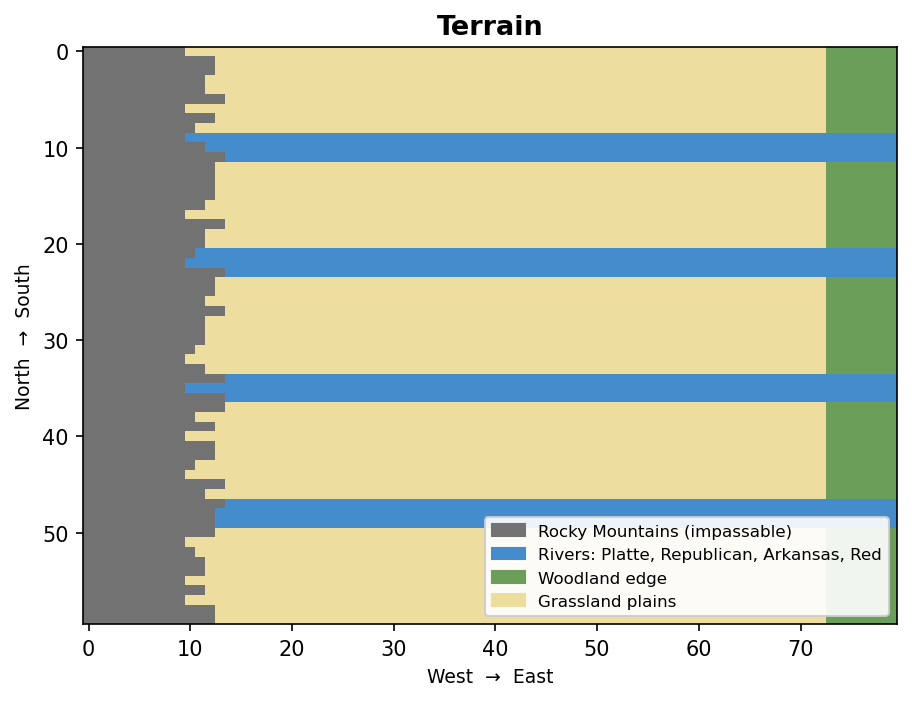
\includegraphics[width=\linewidth]{fig_terrain.png}
    \end{column}
  \end{columns}
\end{frame}

% ── Terrain ──────────────────────────────────────────────────────────────────
\begin{frame}{The Grid \& Terrain}
  \begin{columns}[T]
    \begin{column}{0.48\textwidth}
      \textbf{Grid:} $60 \times 80$ cells\\
      Row~0 = North \quad Col~0 = West
      \vspace{0.8em}

      \begin{tabular}{@{}lp{5cm}@{}}
        \toprule
        Terrain & Notes \\
        \midrule
        Mountains & Western $\sim$12 cols; impassable barrier;
                    jagged edge ($\pm2$ cols/row) \\[4pt]
        Rivers    & 4 E-W bands at fixed rows; higher resource cap (1.4 vs 1.0);
                    approximate Platte, Republican, Arkansas, Red \\[4pt]
        Woodland  & Eastern $\sim$7 cols; lower resource cap (0.75);
                    settlers' entry point \\[4pt]
        Plains    & Remainder; standard resource cap (1.0) \\
        \bottomrule
      \end{tabular}
    \end{column}
    \begin{column}{0.48\textwidth}
      \centering
      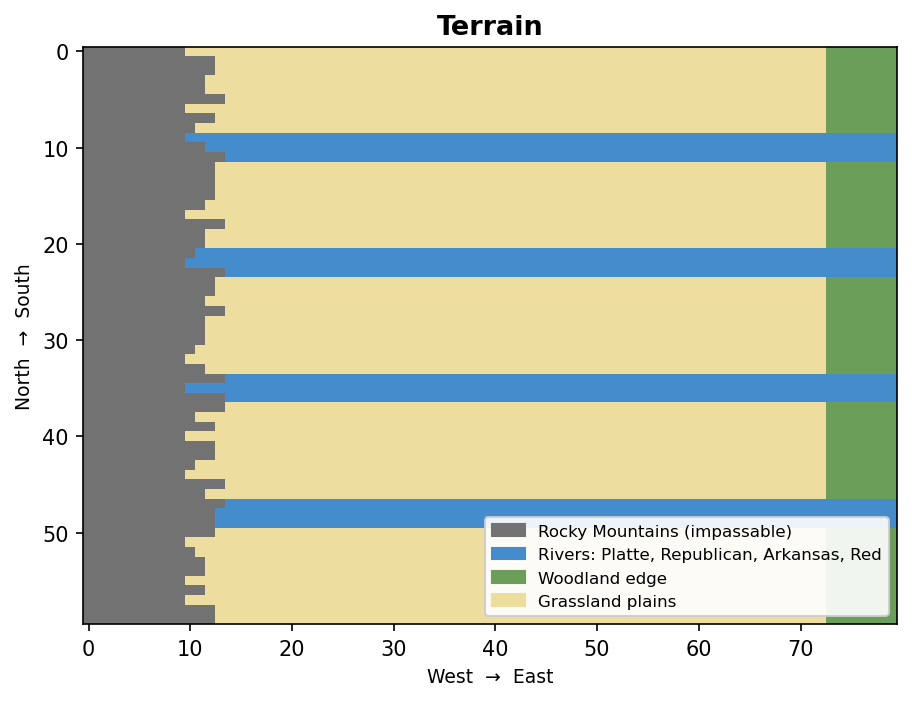
\includegraphics[width=\linewidth]{fig_terrain.png}
    \end{column}
  \end{columns}
\end{frame}

% ── State layers ─────────────────────────────────────────────────────────────
\begin{frame}{Model State}
  Four 2-D arrays evolve each step:
  \vspace{0.5em}

  \begin{tabular}{@{}llp{7cm}@{}}
    \toprule
    Layer & Units & Description \\
    \midrule
    \texttt{resources}  & $[0,\,C]$ &
      Combined grass/water abundance; $C$ varies by terrain \\[4pt]
    \texttt{wildlife}   & count &
      Bison population density; starts as Gaussian blob centred in plains \\[4pt]
    \texttt{humans}     & count &
      Settler population density; starts along the eastern woodland edge \\[4pt]
    \texttt{infra}      & $[0,\,1]$ &
      Infrastructure (trails, towns); grows with human presence,
      decays when settlers leave \\
    \bottomrule
  \end{tabular}

  \vspace{0.8em}
  Every array is multiplied by a static \textbf{mask} (0 on mountains, 1
  elsewhere) after each update, so mountains stay permanently empty.
\end{frame}

% ── Flux: weights ────────────────────────────────────────────────────────────
\begin{frame}{The Flux Mechanism — Directional Weights}
  For each cell $(i,j)$ and each cardinal direction $d \in \{N,S,E,W\}$:
  \vspace{0.4em}

  \begin{block}{Attractiveness \& softmax weights}
    \[
      a_d(i,j) \;=\; \text{attractiveness of the neighbour in direction } d
    \]
    \[
      w_d \;=\; \exp\!\bigl(\beta\cdot a_d\bigr)\cdot
                \mathbf{1}[\text{neighbour is passable}]
    \]
    \[
      f_d \;=\; \frac{w_d}{\displaystyle\sum_{d'} w_{d'}},
      \qquad \sum_d f_d = 1
    \]
  \end{block}

  \begin{itemize}
    \item $\beta$ = \texttt{drift\_strength}: large $\beta$ $\Rightarrow$ decisive
          gradient-following; small $\beta$ $\Rightarrow$ diffusive random walk
    \item Invalid neighbours (mountains, grid boundary) get $w_d = 0$, so
          population never flows into them
    \item Normalisation to 1 \textbf{guarantees mass conservation} during movement
    \item Attractiveness for \emph{wildlife}: resources only\\
          Attractiveness for \emph{humans}: weighted blend of resources +
          infrastructure
  \end{itemize}
\end{frame}

% ── Flux: outflow ─────────────────────────────────────────────────────────────
\begin{frame}{The Flux Mechanism — Outflow \& Inflow}
  \begin{block}{Total outflow from cell $(i,j)$}
    \[
      \mathrm{out}(i,j) \;=\;
        \min\!\Bigl(P,\;
          r_b\,P \;+\; r_p\,\max\!\bigl(0,\,P - K\bigr)
        \Bigr)
    \]
  \end{block}

  \begin{tabular}{@{}cl@{}}
    $P$   & local population \\
    $r_b$ & \texttt{base\_flux} — baseline restlessness each step \\
    $r_p$ & \texttt{pressure\_rate} — extra outflow per unit above $K$ \\
    $K$   & \texttt{carrying\_cap} — pressure threshold (not a hard ceiling) \\
  \end{tabular}

  \vspace{0.8em}
  Directed outflow: $\;\mathrm{out}_d = \mathrm{out}\cdot f_d$

  \vspace{0.4em}
  \textbf{Inflow} at $(i,j)$ = sum of directed outflows from each of the four
  neighbours pointing toward $(i,j)$, computed by shifting the outflow arrays
  by one cell.

  \vspace{0.4em}
  \textbf{Net delta} $= \mathrm{inflow} - \mathrm{outflow}$, then multiplied by
  mask.
\end{frame}

% ── Other dynamics ────────────────────────────────────────────────────────────
\begin{frame}{Other Per-Step Dynamics}
  \begin{columns}[T]
    \begin{column}{0.48\textwidth}
      \textbf{Resource regeneration (logistic)}
      \[
        \Delta R = r_\mathrm{regen}\cdot R\cdot\!\left(1 - \frac{R}{C}\right)
      \]
      Fast recovery when depleted; slows near cap $C$.

      \vspace{0.8em}
      \textbf{Climate events (per step)}
      \begin{itemize}
        \item Drought: prob.\ 0.025, radius 9, severity 0.55
        \item Fire: prob.\ 0.012, radius 5, severity 0.70
        \item Epicentre chosen at random; Gaussian damage footprint
        \item Resources multiplied by $(1 - \mathrm{damage})$
      \end{itemize}
    \end{column}
    \begin{column}{0.48\textwidth}
      \textbf{Logistic birth / death}
      \[
        \Delta P_+ = r_+\cdot P\!\left(1 - \frac{P}{K}\right), \quad
        \Delta P_- = r_-\cdot P
      \]

      \vspace{0.4em}
      \textbf{Consumption (grazing / settlement)}
      \[
        \Delta R_{\mathrm{consumed}} = \min\!\bigl(R,\; P\cdot c\bigr)
      \]
      Bison graze \emph{before} settlers consume, so they compete
      for the same pool within a step.

      \vspace{0.6em}
      \textbf{Infrastructure}
      \[
        \Delta I = g\,\frac{P}{K} - d\,I\!\left(1 - \frac{P}{K}\right)
      \]
      Towns grow with density; decay slowly when abandoned.
    \end{column}
  \end{columns}
\end{frame}

% ── Update order ─────────────────────────────────────────────────────────────
\begin{frame}{Update Order Each Step}
  Order matters — populations respond to the \emph{current} landscape:

  \vspace{0.5em}
  \begin{enumerate}
    \item \textbf{Resource regeneration} — logistic recovery toward terrain cap
    \item \textbf{Climate event} — stochastic drought or fire (or neither)
    \item \textbf{Wildlife update} — flux + birth/death + grazing
    \item \textbf{Human update} — flux + birth/death + consumption\\
          \hspace{2em}{\small(sees resources already depleted by bison)}
    \item \textbf{Infrastructure update} — towns grow/decay based on human density
    \item \textbf{Record snapshot} (every \texttt{record\_every} steps)
  \end{enumerate}

  \vspace{0.6em}
  All state arrays are updated \textbf{synchronously} from the previous
  step's values — standard CA practice that avoids order-of-operations
  artefacts within a step.
\end{frame}

% ── Initial state ─────────────────────────────────────────────────────────────
\begin{frame}{Initial State  ($t = 0$)}
  \centering
  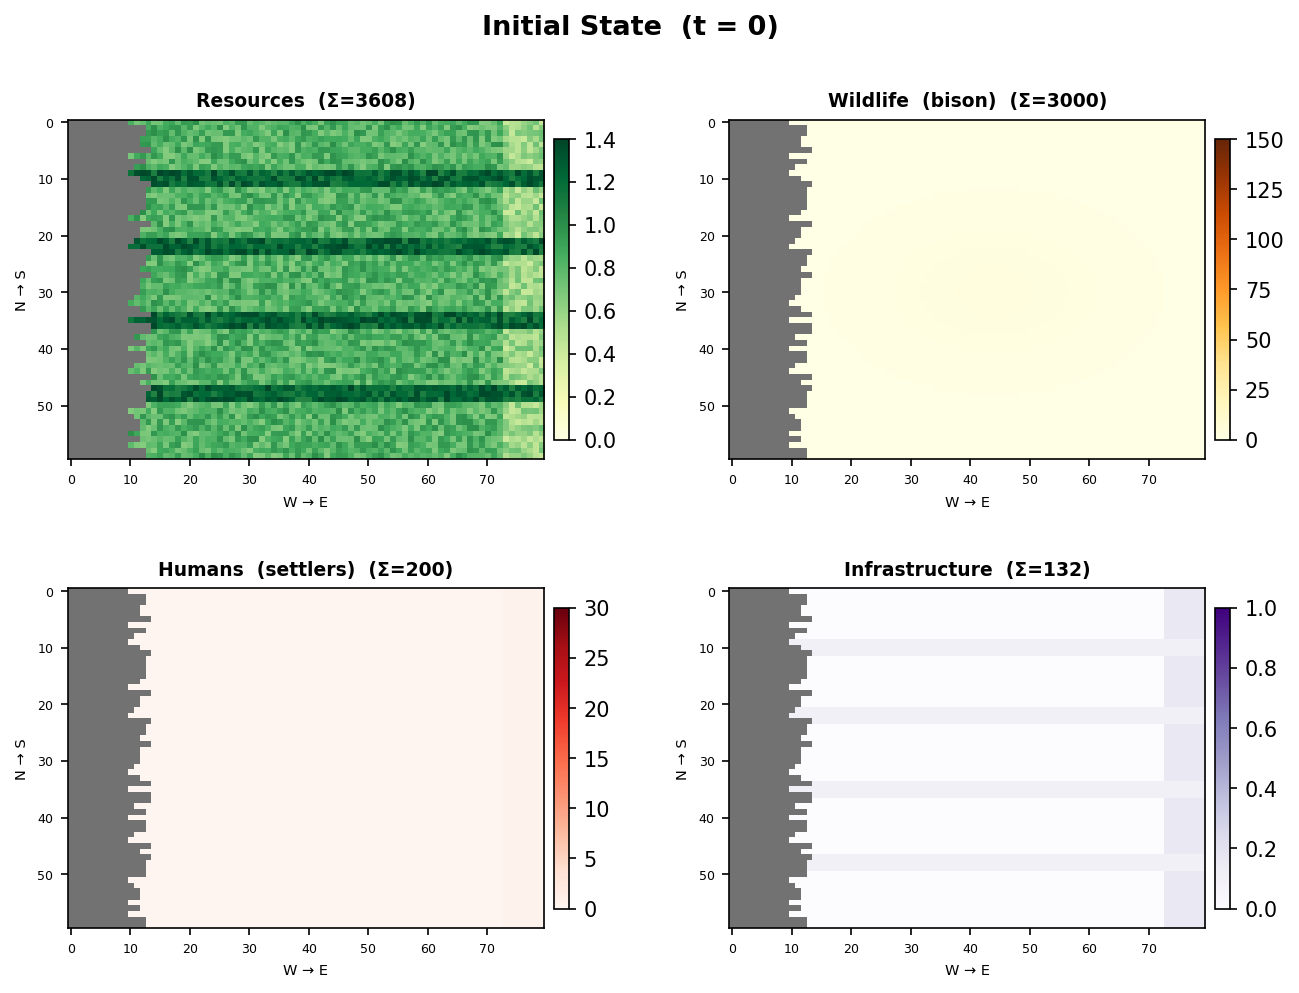
\includegraphics[width=0.82\linewidth]{fig_t0.png}
\end{frame}

% ── Final state ───────────────────────────────────────────────────────────────
\begin{frame}{After 200 Steps  ($t = 200$)}
  \centering
  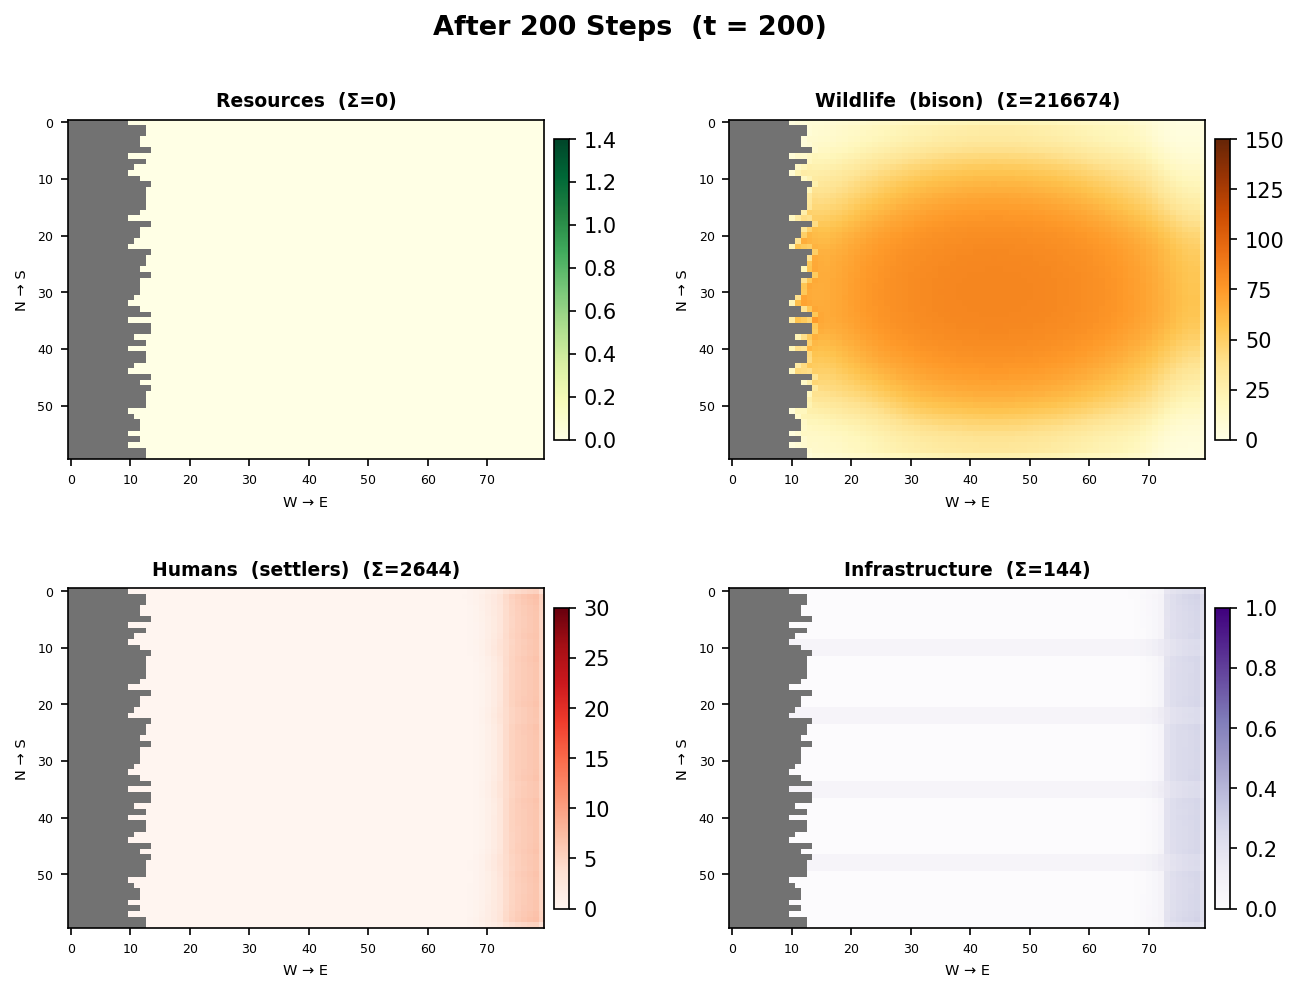
\includegraphics[width=0.82\linewidth]{fig_t200.png}
\end{frame}

% ── History ───────────────────────────────────────────────────────────────────
\begin{frame}{Population \& Resource History}
  \centering
  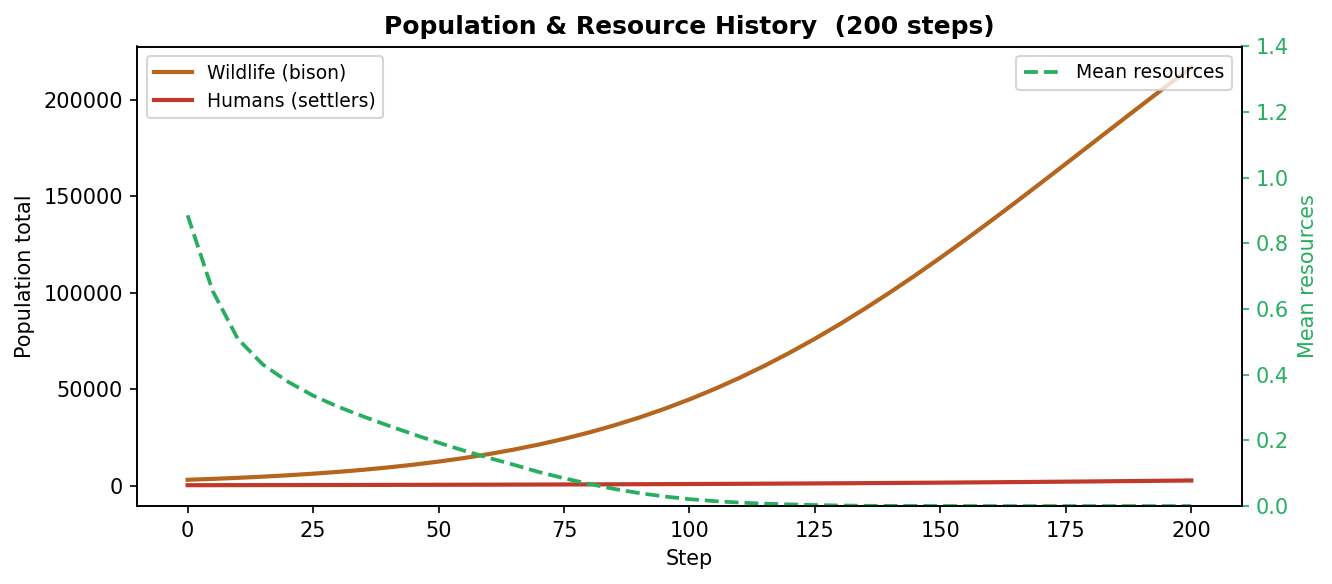
\includegraphics[width=0.90\linewidth]{fig_history.png}

  \vspace{0.3em}
  \small
  Bison outpace the grassland's recovery rate and crash resources by $\sim$step 75.\\
  Settlers remain sparse — their slower dynamics are masked by the bison explosion.
\end{frame}

% ── Known dynamics & next steps ───────────────────────────────────────────────
\begin{frame}{Known Dynamics \& Next Steps}
  \begin{columns}[T]
    \begin{column}{0.48\textwidth}
      \textbf{Current behaviour (default params)}
      \begin{itemize}
        \item Bison undergo exponential growth then resource crash by $\sim$step 75
        \item Settlers grow slowly; swamped by bison in resource competition
        \item Infrastructure seeds along rivers and woodland edge but spreads slowly
      \end{itemize}

      \vspace{0.5em}
      \textbf{Tuning levers for stable dynamics}
      \begin{itemize}
        \item Lower \texttt{wl\_consumption} (less aggressive grazing)
        \item Raise \texttt{res\_regen\_rate} (faster grassland recovery)
        \item Lower \texttt{wl\_carrying\_cap} (earlier pressure to disperse)
      \end{itemize}
    \end{column}
    \begin{column}{0.48\textwidth}
      \textbf{Planned extensions}
      \begin{itemize}
        \item Wildlife--human repulsion (bison flee settler-dense cells)
        \item Seasonal resource variation (modulate regrowth rate by season)
        \item Historical scenario mode (introduce railroads, hunting pressure
              at specific steps)
        \item Spatially correlated initial resources (gaussian-blurred noise)
        \item Finer inline comments inside \texttt{\_flux()} method
      \end{itemize}

      \vspace{0.5em}
      \textbf{Code}\\
      \small
      Single file: \texttt{plains\_ca.py}\\
      All parameters in top-level \texttt{PARAMS} dict\\
      Output: \texttt{results/YYYYMMDDhhmm\_*.png/json}
    \end{column}
  \end{columns}
\end{frame}

\end{document}
